\subsubsection{Architecture}
\begin{itemize}
    \item Comprise 1 GK110 GPU\cite{gpu_specs}.
    \item 6 GB of GDDR5 on-board memory\cite{gpu_specs}.
    \item 2688 cores\cite{gpu_specs}.
    \item 732MHz speed clock per core\cite{gpu_specs}.
    \item 15 SMX units, each of these contains 192 single-precision cores\cite{gpu_specs1}.
    \item The SMX schedules threads in groups of 32 parallel threads calles \emph{warps}. Each SMX features 4 \emph{warp}
        schedulers and 8 instruction dispatch units, allowing 4 warps to be issued and executed concurrently\cite{gpu_specs1}.
    \item 64 KB Configurable Shared Memory and L1 Cache and 48KB Read‐Only Data Cache\cite{gpu_specs1}.
    \item 1536KB of dedicated L2 cache memory\cite{gpu_specs1}.
    \item 32 Threads per Warp\cite{gpu_specs1}.
    \item Maximum numbers of Warps per Multiprocessor 64\cite{gpu_specs1}.
    \item Maximum numbers of threads per Multiprocessor 2048\cite{gpu_specs1}.
    \item Maximum numbers of thread blocks per Multiprocessor 16\cite{gpu_specs1}.
    \item 65536 32-bit registers per Multiprocessor\cite{gpu_specs1}.
    \item Maximum number of registers per thread 255\cite{gpu_specs1}.
    \item Maximum number of threads per thread block 1024\cite{gpu_specs1}.
    \item Shared memory size configurations 16K, 32K and 48K\cite{gpu_specs1}.
\end{itemize}

\par{Figure \ref{GpuArch} Shows a global view of the GK110 gpu architecture.}

\begin{figure}[!h]
    \centering
    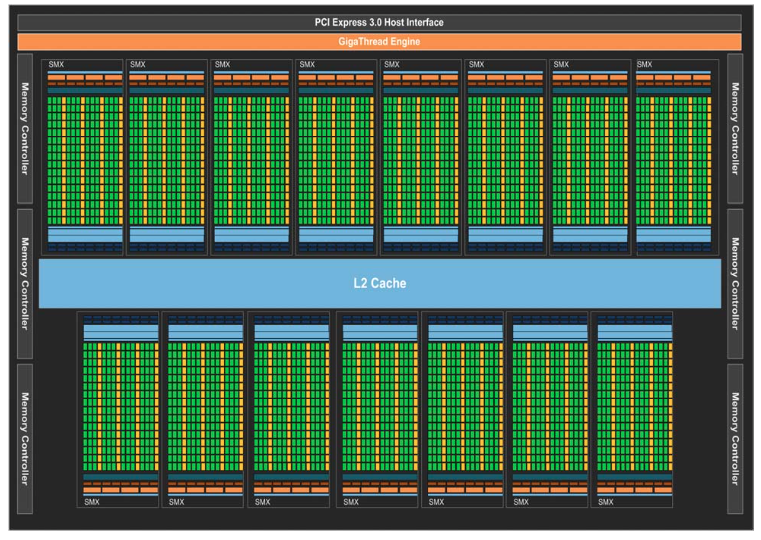
\includegraphics[width=0.5\textwidth]{figures/gpu_arch.png}
    \caption{Kepler GK110 architecture\cite{gpu_specs1}.}
    \label{GpuArch}
\end{figure}

\subsubsection{Mapping}
\begin{itemize}
    \item The CUDA architecture is a scalar architecture. Therefore, there is no performance benefit from using vector types and 
        instructions\cite{gpu_opencl_cuda}.
    \item A \emph{work item} is executed on a scalar processor\cite{gpu_opencl_opt_slides}.
    \item \emph{Work groups} are executed on multiprocessors(SMX)\cite{gpu_opencl_opt_slides}.
    \item Only one \emph{kernel} can execute in a device at one time\cite{gpu_opencl_opt_slides}.
    \item \emph{Work groups} divide into groups of 32 threads called warps. Warps always perform the same instruction and they
        are basic scheduling units\cite{gpu_opencl_opt_slides}.
    \item OpenCL private memory is implemented as registers in the GPU\cite{gpu_opencl_opt_slides}.
    \item OpenCL local memory is implemented as shared memory in the GPU\cite{gpu_opencl_opt_slides}.
    \item If branching happens within a warp, different execution paths must be serialized, increasing the total number of 
        instructions although there is no penalty if different warps diverge\cite{gpu_opencl_opt_slides}.
\end{itemize}

\begin{figure}[!h]
    \centering
    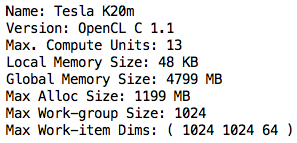
\includegraphics[width=0.35\textwidth]{figures/gpu_device_info.png}
    \caption{GPU device information.}
    \label{GpuDeviceInfo}
\end{figure}

\par{..\cite{gpu_specs1}\ref{GpuDeviceInfo}\cite{gpu_opencl_cuda}}




